\chapter{Les Projets}
\label{Developpement}

\section{MobiSAAS}

\subsection{Cahier des charges}

\subsubsection{Présentation des besoins}

Le projet \og MobiSAAS \fg : MobiAnalyst as a Service, s'inscrit dans la démarche d'entreprise de proposer des solutions en mode \textbf{SAAS}. Le projet consiste d'une manière générale à exposer les fonctionnalités de la solution Desktop du produit \og MobiAnalyst\footnote{\url{http://www.mobianalyst.fr/}} \fg. C'est pour ce projet que j'ai effectué mon travail de stage. \\

\begin{figure}[!h]
\centering
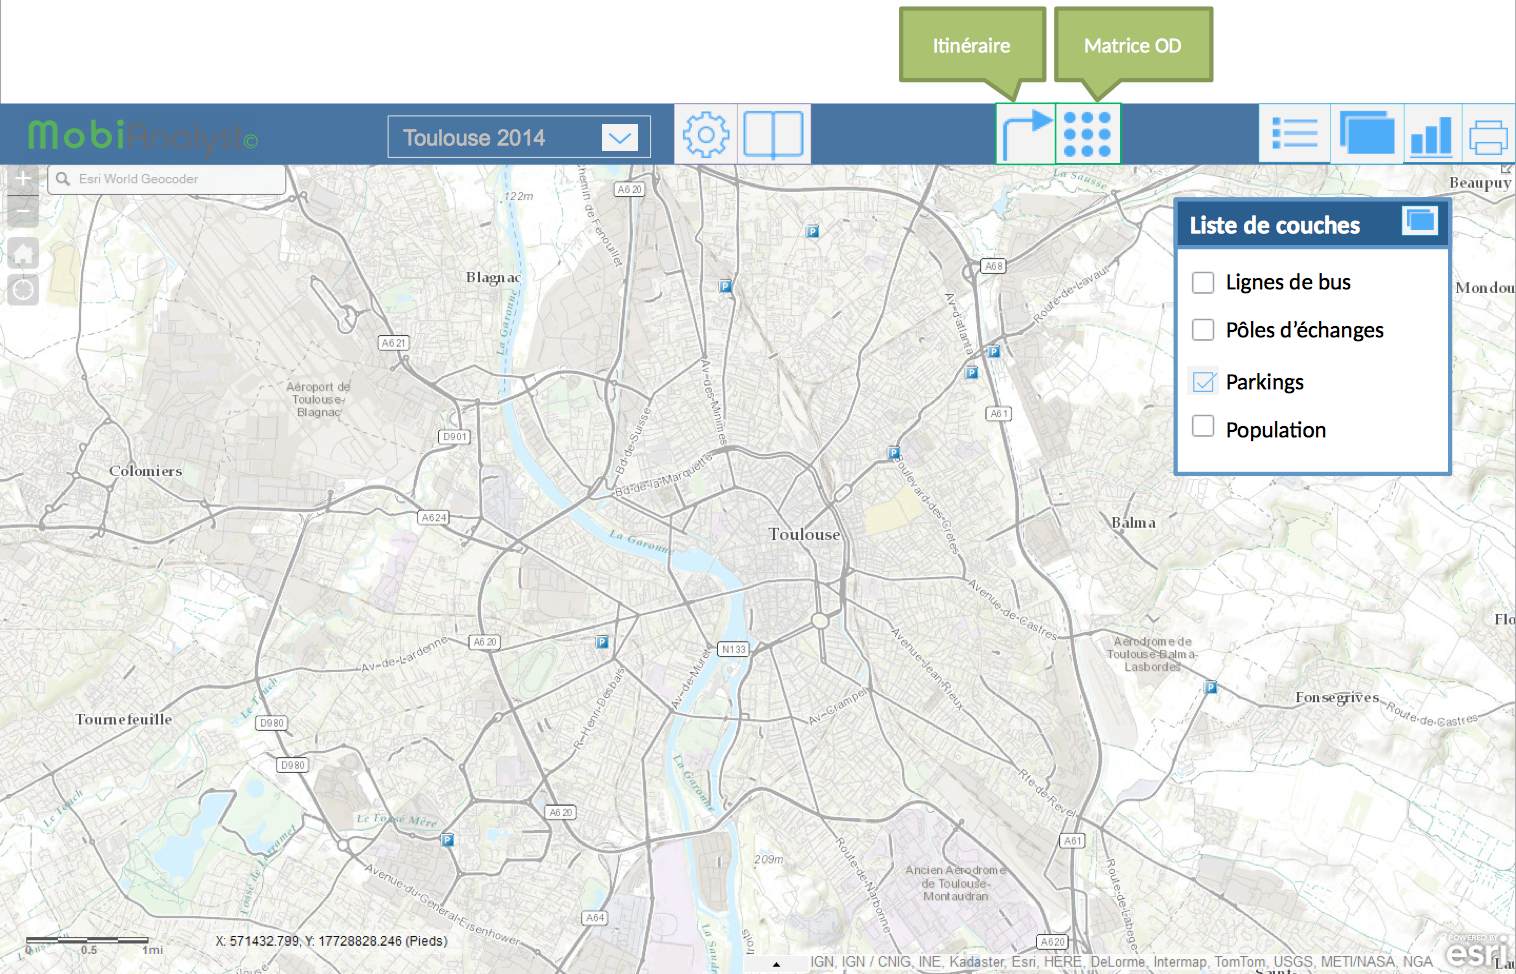
\includegraphics[width=16cm]{images/MobiSAAS_IHM.png}
\caption{\label{MobiSAAS_IHM.png}Interface de MobiSAAS (frontend)}
\end{figure} 
\\


Mon sujet de stage porte sur le développement de \textbf{web services} permettant d'exposer des fonctionnalités d'importation de données voirie et transport en commun, pour la construction automatique de réseaux de transports multi-modaux (graphes)(Fig. \ref{OffreMobiAnalyst}). \\

\begin{figure}[h]
\centering
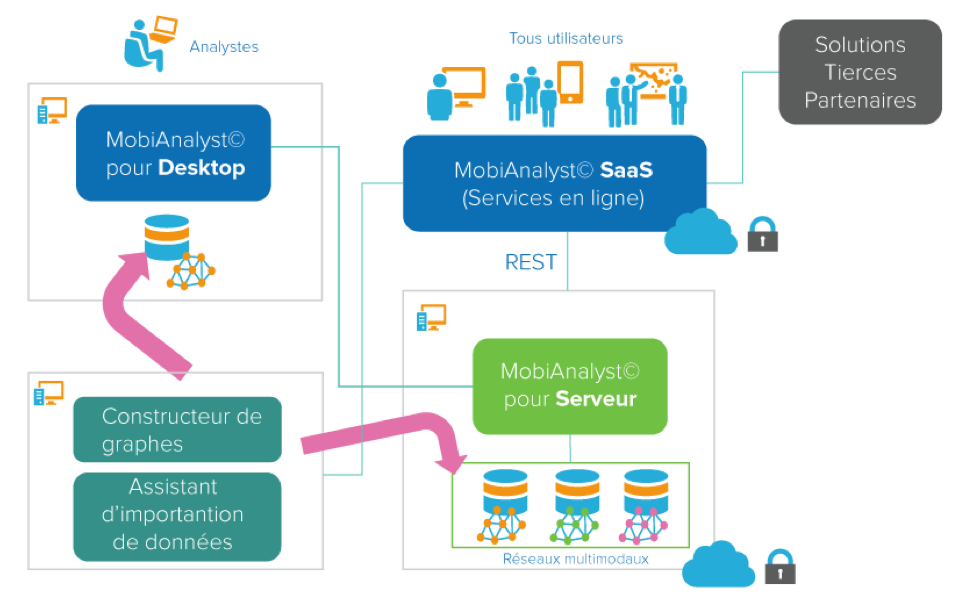
\includegraphics[width=16cm]{images/offre_MobiAnalyst.png}
\caption{\label{OffreMobiAnalyst}Offres du produit MobiAnalyst}
\end{figure} 
\\

Les serveurs MobiAnalyst propose une \textbf{API} de services web de type \textbf{REST} avec des fonctions bas niveau :
\begin{itemize}
\item Calcul d'un itinéraire multi-modal 
\item Calcul d'un isochrone multi-modal
\item Calcul d'une MOD
\item Géotraitements d'analyse réseaux 
\end{itemize}

C'est dans le cadre de l'interface d'administration de l'application (backend) que je devais développer des fonctionnalités d'upload de données de transport (GTFS\footnote{\url{https://developers.google.com/transit/gtfs/}}) sur le serveur.\\

L'objectif de mon travail a été d'exposer des fonctionnalités (en vert sur Fig. \ref{OffreMobiAnalyst}) codées initialement en langage SQL et/ou Python via une API REST en langage Java (JAX-RS). 

J'ai donc dans un premier temps pris en main les chaînes de traitements (Python) et appris à manipuler les données (Postgis/SQL) via le projet \og DataWizard \fg. En parallèle, afin d'implémenter ces web services j'ai intégré le projet « MobiSAAS » et ainsi appris à développer avec le framework \og Dropwizard \fg. \\

\subsubsection{Une API REST ?}

J'ai tout d'abord découvert ce qu'est une API REST et surtout comment la concevoir (maquetter). Je me suis inspiré de l'article suivant :\\
\url{http://blog.octo.com/designer-une-api-rest/ } dont voici les grands principes à retenir :

\begin{itemize}
\item REST est un style d'architecture orienté ressource (ROA).
\item L'abstraction clé de l'information en REST est une « Ressource ». N'importe quelle information qui peut être nommée est une ressource : une image, un document, un service temporel (la météo d'aujourd'hui à Toulouse), une collection d'autres ressources, un objet physique (une personne) etc. En d'autres termes, n'importe quel concept qui peut être la cible d'une référence d'un lien hypertexte doit s'adapter dans la notion de ressource.
\item L'API doit donc proposer des web services sur ces ressources qui répondent aux requêtes du protocole HTTP (GET, POST, PUT, DELETE).
\item Le concept de représentation (XML/JSON) est important. Nous avons choisi de ne représenter les résultats de requêtes (Response) que via le format d'échange de données JSON (JavaScript Object Notation).
\item Une dernier concept fondamental sont les réponses de ces services. Le WS peut renvoyer des données (JSON), et des codes HTTP (\url{https://fr.wikipedia.org/wiki/Liste_des_codes_HTTP}). Il est préconisé d'utiliser les codes de retour HTTP (500, 404, 200), de manière appropriée, sachant qu'il existe un code pour chaque cas d'utilisation courant. Ces codes sont connus de tous. 
\end{itemize}

\subsubsection{Architecture actuelle}

La figure \ref{fig:architectureMobiAdmin} détaille l'ensemble des briques logicielles nécessaires au fonctionnement de la plate-forme MobiSAAS :
\begin{itemize}
\item \textbf{AGS} : ArcGIS Server. Le serveur de Système d'Information Géographique (SIG) permettant de publier et d'administrer des services cartographiques (MapService).
Dans notre cas, les MapServices déployés sont des réseaux routiers et de transport en commun (TC), accompagnés de tables horaires (TimeTable) contenant les horaires des TC.
\item \textbf{SOE}: Server Object Extension. Nous utilisons le mécanisme d'extension \og SOE \fg pour déployer sur un MapService un service spécifique à MobiSAAS. Un SOE est une fonctionnalité qui se déploie sur un MapService et qui expose en Web Service (REST ou SOAP) les solveurs (algorithme de résolution d'itinéraires) de MobiAnalyst.
\item \textbf{MobiAdmin}: Serveur REST d'administration MobiSAAS. Ce serveur (basé sur Java) est le point d'entrée des utilisateurs des services REST de MobiAnalyst.
Il redirige les requêtes métiers vers le bon SOE déployé, il trace ces requêtes et enrichit la base de données client de MobiAnalyst.
L'authentification qui est faite dans les requêtes utilise les comptes d'AGS créés au préalable.
\item \textbf{Postgres} : Système de gestion de base de données. Cette base contient les données clients de MobiAnalyst : profil, traces d'utilisation de MobiSAAS.
\item \textbf{MongoDB} : Système de gestion de base de données. Cette base contient les logs (statistiques mesurées en temps réel) correspondant aux services REST de MobiSAAS.
\end{itemize}\\

\begin{figure}[!h]
	\centering
		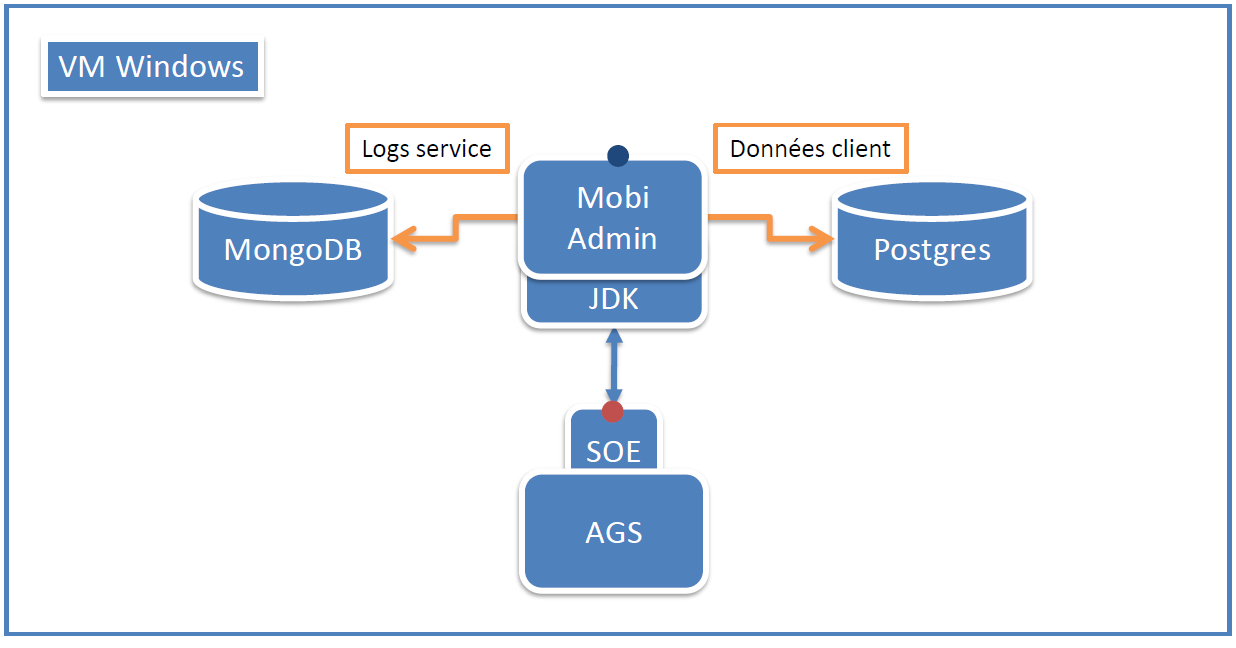
\includegraphics[width=0.8\textwidth]{images/architecture.png}
	\caption{Architecture globale de \og MobiAdmin \fg}
	\label{fig:architectureMobiAdmin}
\end{figure}\\

\subsection{Eléments de spécifications fonctionnelles}

Mon stage et les développements demandés concernent le composant d'administration de l'infrastructure : \og MobiAdmin \fg (cf. Fig. \ref{fig:architectureMobiAdmin}). Dans l'objectif de gérer les données du client, je dois proposer un web service pour la gestion des données de transport dans l'espace privatif du client.
La fonctionnalité principale à développer est donc un web service d'upload de données et plus particulièrement l'upload de données de transport public au format GTFS\footnote{\url{https://developers.google.com/transit/gtfs/reference}}.\\ 

Les données GTFS se présentent le plus souvent dans une archive contenant au minimum les 8 fichiers .txt suivants :
\\
\begin{figure}[h]
	\centering
		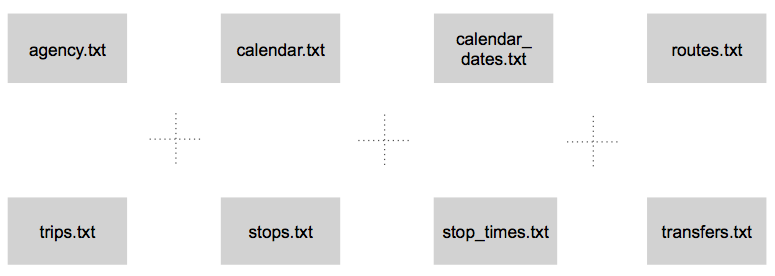
\includegraphics[width=0.8\textwidth]{images/GTFS_8fichiers.png}
	\caption{Contenu des données GTFS}
	\label{fig:GTFS_8fichiers}
\end{figure}\\


L'objectif de ce service d'import de données GTFS est de pouvoir manipuler ces données (fichier au format zip), et de récupérer des métadonnées. Par exemple : l'extension géographique des données, le nom de l'agence, le nombre de lignes, le mode de transport, etc. L'objectif final est de publier un réseau de transport en commun via un service en ligne. Actuellement, ces fonctionnalités sont réalisées en amont du logiciel MobiAnalyst via le logiciel Desktop DataWizard (cf. \ref{DataWizard} DataWizard).\\

Une archive ou  \og Upload \fg de données GTFS peut contenir un seul ou plusieurs jeu(x) de données (ensemble de fichiers .txt). Il faut donc récupérer et renseigner les métadonnées de chaque Upload sur le serveur :
\begin{itemize}
\item Nom - UUID (identifiant unique)
\item Date d'upload
\item Status d'upload (SUCCESS, FAILED, LOADING, INIT)
\item Nom de l'archive (source)
\item Chemin vers le rapport de validation GTFS
\item Chemin vers la données

\end{itemsize}\\
~\\
Les résultats attendus sont le stockage sur le serveur (système de fichier) des données envoyées par le client, la trace de l'opération dans un SGBD, et enfin la production de réponses HTTP (format JSON) pour chaque requête sur le service. 

Les étapes successives du traitement seront donc : le téléchargement de l'archive sur le serveur, la validation des données, et enfin le chargement en base.\\

Pour les besoins de cette API nous avons spécifié des codes d'erreurs propres à l'application et au contexte : 601, 602, 603, respectivement Upload Failed, Validation Failed, Loading Failed.\\

Ce service dédié aux données GTFS est très spécifique. Une attention particulière a été faite afin de développer de manière à abstraire et rendre au maximum générique la plupart des composants afin de proposer d'autres format de données à l'importation sur le serveur REST \og MobiAdmin \fg (utilisation d'interfaces et de classes abstraites pour la mise en place de l'héritage).\\


\subsection{Eléments de spécifications techniques}

Pour le composant \og MobiAdmin \fg (serveur REST) qui va héberger les services, le choix technologique majeur est d'utiliser le framework DropWizard (cf. \ref{Dropwizard}). Ce framework orienté microservices nous permet de fournir notamment un serveur embarqué HTTP \og Jetty \fg. Et le framework open source Jersey pour la partie webservice REST qui est l'implémentation de référence de la spécification JAX-RS. Ou encore la librairie Jackson \og King of JSON \fg pour la sérialisation/désérialisation du JSON.\\

L'environnement de développement est donc un projet Java EE Maven (cf. \ref{Maven}) composé des éléments de Dropwizard. 
Les \textbf{WS} exposés sont à priori \og lourds \fg, sachant qu'un jeu de données peut faire jusqu'à plusieurs centaines de Mo, les opérations de téléchargement, validation, traitement, stockage peuvent être long à répondre au client après chaque requête. Les WS à développer sont donc asynchrones. 
Chaque requête renvoie une réponse \og immédiatement \fg pendant que le processus (thread) continu de s'effectuer afin de produire un résultat. A l'aide d'une Map (UploadMap), chaque requête GET (by ID) renvoie le status de l'opération : \og en cours \fg, ou \og ok \fg. Si l'opération ne se déroule pas complètement une exception est levée et renvoie un des 3 codes d'erreurs. Le client peut par exemple effectuer des requêtes simultanément (GET) afin de demander le status de son upload. De plus, une contrainte supplémentaire est que le service doit supporter plusieurs requêtes simultanées, il faudra donc s'orienter vers un développement en mode \og programmation concurrente \fg. Pour cela, on utilise le framework \og executor \fg avec notamment l'interface \og Callable \fg et un objet \og newFixedThreadPool \fg (cf. \ref{Threads}). \\

\pagebreak

\subsubsection{Technologies utilisées}\label{MobiSAASTechno}

\textbf{Apache Maven : } \label{Maven}

\begin{wrapfigure}{l}{3cm}
\centering

\includegraphics[width=3cm]{images/apacheMaven.jpg}
\end{wrapfigure}
\noindent C'est un outil pour la gestion et l'automatisation de production des projets logiciels Java en général et Java EE en particulier. L'objectif recherché est comparable au système Make sous Unix : produire un logiciel à partir de ses sources, en optimisant les tâches réalisées à cette fin et en garantissant le bon ordre de fabrication.\\
Il est semblable à l'outil Ant, mais fournit des moyens de configuration plus simples, eux aussi basés sur le format XML. Maven est géré par l'organisation Apache Software Foundation. Précédemment Maven était une branche de l'organisation Jakarta Project.\\
Maven utilise un paradigme connu sous le nom de Project Object Model (\textbf{POM}) afin de décrire un projet logiciel, ses dépendances avec des modules externes et l'ordre à suivre pour sa production. Il est livré avec un grand nombre de tâches pré-définies, comme la compilation de code Java ou encore sa modularisation.\\
Un élément clé et relativement spécifique de Maven est son aptitude à fonctionner en réseau. Une des motivations historiques de cet outil est de fournir un moyen de synchroniser des projets indépendants : publication standardisée d'information, distribution automatique de modules « jar ». Ainsi en version de base, Maven peut dynamiquement télécharger du matériel sur des dépôts logiciels connus. Il propose ainsi la synchronisation transparente de modules nécessaires.\\

Dans le projet MobiSAAS, Maven est très utilisé car c'est un projet multi-modules avec un module parent. Maven me permet donc de télécharger et de gérer les dépendances du projet. Par exemple, voici une extrait du fichier \textbf{POM} du module utilitaire \og mobi-admin-util \fg que j'ai développé (Fig. \ref{fig:MavenPOM}).\\

\begin{figure}[!h]
	\centering
		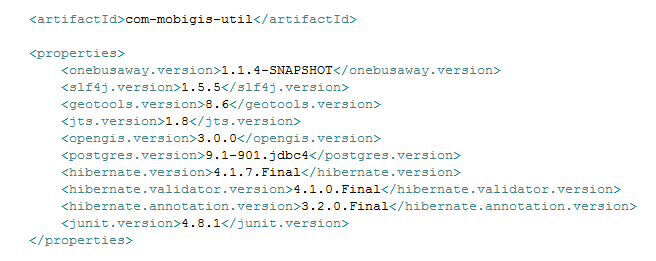
\includegraphics[width=0.8\textwidth]{images/Maven_POM_properties_Mobi-Admin-util.PNG}
	\caption{\label{fig:MavenPOM}Extrait du fichier POM, versions des dépendances utilisées}
\end{figure}
\\
~\\
\textbf{Dropwizard :}\label{Dropwizard}

\begin{wrapfigure}{l}{3cm}
\centering

\includegraphics[width=3cm]{images/dropwizard.png}
\end{wrapfigure}
\noindent C'est un framework Java léger adapté au développement rapide de microservices REST et ne nécessitant pas de serveur d'application comme environnement d'exécution.
Cela dit, au delà du framework, c'est surtout un assemblage habile de composants spécialisés parmi les meilleurs de l'écosystème Java :
~~\\
~~\\
\begin{itemize}
\item \textbf{Jetty}, un serveur HTTP et un moteur de servlet
\item \textbf{Jersey}, l'implémentation de référence de la spécification JAX-RS (web services REST) 
\item \textbf{Jackson}, une librairie de sérialisation/dé-sérialisation JSON 
\item \textbf{Hibernate Validator}, l'implémentation de référence de l'API Bean Validation (JSR 303) 
\item \textbf{SLF4J} et \textbf{Logback} pour la gestion des traces 
\item \textbf{Metrics} pour le monitoring 
\item \textbf{jDBI} pour l'interfaçage rapide à une base de données relationnelle. Cette librairie est de bien plus bas niveau que JPA ou Hibernate et présente peu d'abstraction ce qui rend sa prise en main aisée \\
\end{itemize}

Packagée sous la forme d'un jar autonome contenant toutes ses dépendances, l'unité de déploiement n'a pas besoin de serveur d'application pour être exécutée (le conteneur Jetty est embarqué dans le jar). Avec ses 10 Mo tout au plus (dépendances comprises) l'empreinte mémoire d'une application Dropwizard est donc incomparablement plus faible qu'un Web Service SOAP déployé dans un serveur d'application Java EE (jusqu'à plusieurs centaines de Mo).
En conséquences, le temps de démarrage d'une application Dropwizard est de quelques secondes quand il faut parfois plusieurs minutes pour un serveur d'application.\\

On peut considérer ce projet comme une alternative crédible aux serveurs d'applications Java EE perçus comme lourds, compliqués et gourmands en ressources. Le champ des applications couvert par Dropwizard est en réalité plus vaste que celui des microservices (il est tout a fait possible de développer une IHM web) mais l'aisance avec laquelle on développe et déploie un service REST en fait une solution très adaptée à ce type d'usage (à l'instar de Spring Boot de Pivotal ou Spark avec lesquels il est en compétition).\\

La structure d'une application Dropwizard de type API RESTful selon les préconisations d'organisation de projet du framework Dropwizard  (cf. Fig ~\ref{Organisation_Dropwizard}) est : 
\\
\begin{figure}[h]
\centering
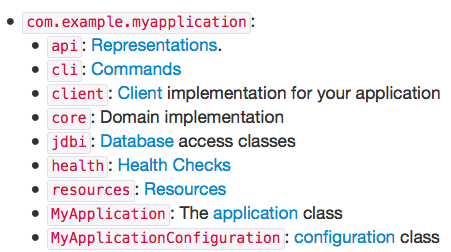
\includegraphics[width=6cm,heigth=6cm]{images/Dropwizard_Project.png}
\caption{\label{Organisation_Dropwizard}Organisation conseillée d'un projet Dropwizard}
\end{figure} 

A partir de cette organisation, nous avons structuré le module \og MobiAdmin \fg comme le montre la figure ci-dessous (cf. Fig ~\ref{Organisation_MobiAdmin}). 
Plusieurs packages spécifiques ou de configuration supplémentaires apparaissent (auth, dao, jsonable, thread,...). 
\\
\begin{figure}[h]
\centering
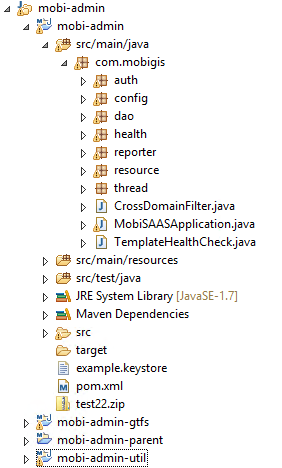
\includegraphics[width=6cm,heigth=6cm]{images/Package_explorer_MobiSAAS.PNG}
\caption{\label{Organisation_MobiAdmin}Organisation du module mobi-admin}
\end{figure} 

\\

\textbf{Hibernate :}

\begin{wrapfigure}{l}{3cm}
\centering

\includegraphics[width=3cm]{images/hibernate.png}
\end{wrapfigure}
\noindent Dans les langages objet, les données étant le plus souvent stockées dans des bases de données relationnelles ainsi l'utilisation d'un framework de mapping Objet/Relationnel est recommandé pour assurer la rapidité, l'évolutivité et la maintenabilité des développements. Hibernate, issu de la communauté Open Source, répond à ce besoin et connaît depuis quelques années un vif succès. Ce succès s'explique notamment par son architecture parfaitement adaptable à tout type de développements et le support de la majorité des bases de données du marché.\\

Afin de développer les classes pour la gestion des données clients (Uploads) du module «mobi-admin». J'ai mis en place une table « mobiuploads » sur le SGBD PostgreSQL (classes Upload.java, UploadDAO.java).
Grâce au framework Dropwizard, nous avons utilisé Hibernate comme ORM (Object Relationnal Mapping). J'ai pu ainsi manipuler mes objets (opérations CRUD) pour la création, la lecture, la mise à jour et la suppression des objets dans la base. 
Egalement, j'ai développé le chargement de ces données métiers (GTFS) dans le SGBD, j'ai mis en place le modèle de données et développé les classes avec les annotations Hibernate (@Entity, @Table, @JoinColumns,...). Ainsi, si le schéma n'existe pas il se génère automatiquement grâce à Hibernate. 
Toutes les requêtes sont écrites dans les classes java en HQL, langage propre à Hibernate grâce aux annotations @NamedQueries. \\


\textbf{Jackson :}

\begin{wrapfigure}{l}{3cm}
\centering
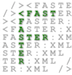
\includegraphics[width=3cm]{images/fxml_logo_Jackson.png}
\end{wrapfigure}
\noindent Jackson est une API JSON, elle est simple, bien documentée, et elle répond aux besoins suivants tels que :
\begin{itemize}
\item Capable de sérialiser et désérialiser des arbres JSON sans adhérence aux beans modèles.
\item Pouvant travailler directement sur des flux.
\item Capable de tenir une charge conséquente, donc stable et performante.
\item Avec le minimum possible de dépendances.
\end{itemize}

Afin que le service puisse renvoyer des réponses convenables et standards nous avons utilisé Jackson via Dropwizard \footnote{\url{http://www.mkyong.com/java/how-to-convert-java-object-to-from-json-jackson/}}. Grâce à la librairie Jackson nous pouvons transformer les \og beans \fg et convertir les propriétés java des objets en éléments Json, ainsi on renvoie par exemple le nom de l'upload, la date d'upload et surtout son status si l'opération s'est bien déroulée ou non (Fig. \ref{fig:Json1}).
\\
\begin{figure}[h]
	\centering
		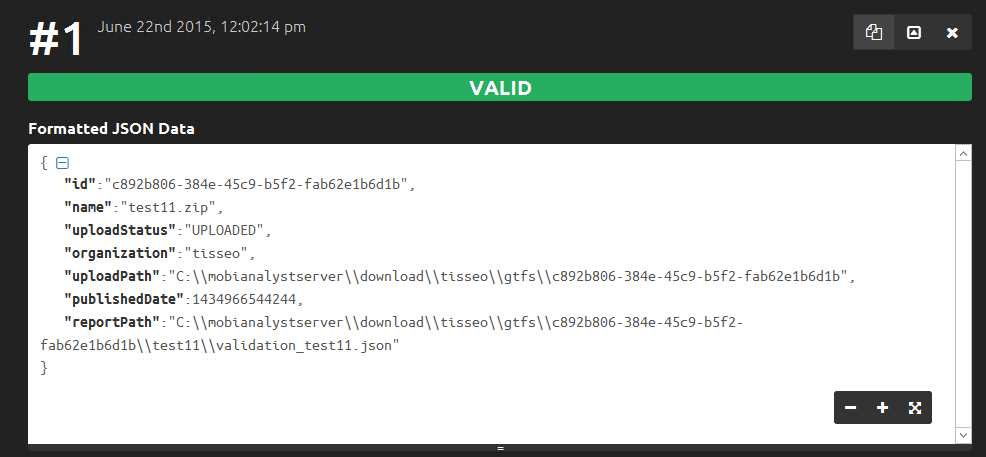
\includegraphics[width=0.8\textwidth]{images/JsonFormatter_serialization.PNG}
	\caption{Réponse Json renvoyée}
	\label{fig:Json1}
\end{figure}\\

De la même manière, chaque donnée GTFS, passe par un traitement métier de validation. Chaque Upload, possède donc une propriété appelée \og reportValidationPath \fg qui indique le chemin vers ce rapport de validation au format json. Ici, Jackson va permettre la production du rapport contenant les métadonnées et les anomalies pour chaque jeu de données GTFS (Fig. \ref{fig:Json2}).
\\
\begin{figure}[h]
	\centering
		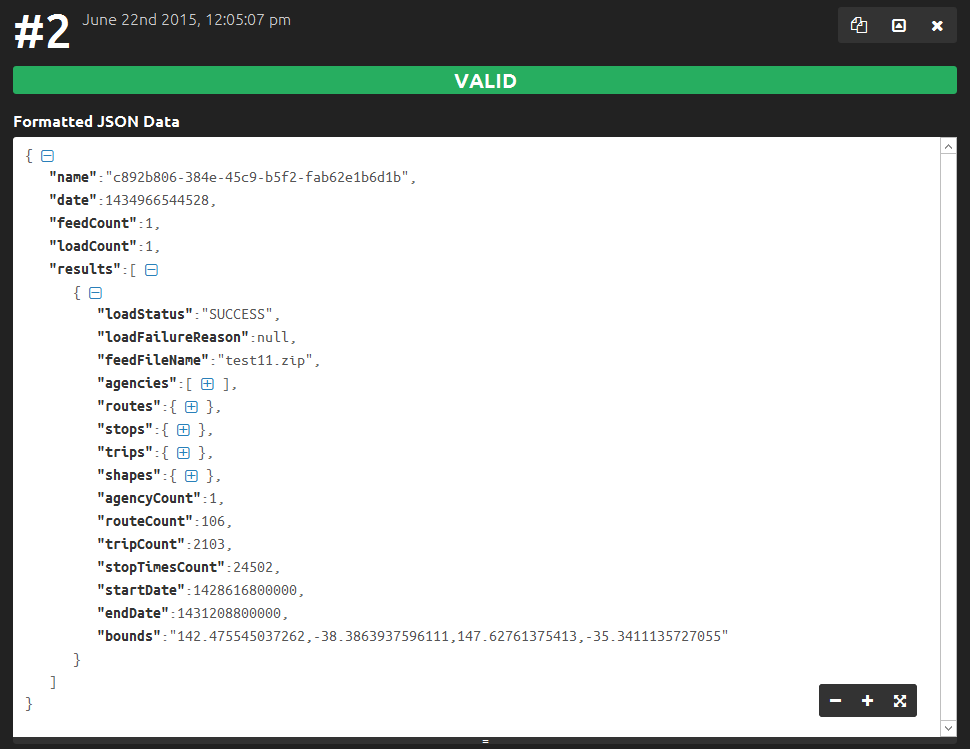
\includegraphics[width=0.8\textwidth]{images/JsonFormatter_serialization_Validation.PNG}
	\caption{Rapport Json de validation des données GTFS}
	\label{fig:Json2}
\end{figure}\\


\textbf{SLF4J et Logback :} 

\begin{wrapfigure}{l}{3cm}
\centering

\includegraphics[width=3cm]{images/slf4j-logo.jpg}

\includegraphics[width=3cm]{images/lblogo.jpg}
\end{wrapfigure}
\noindent SLF4J est une couche d'abstraction pour les API de journalisation Java. Le principe est à peu près similaire à celui de Jakarta Commons Logging. Les avantages de l'utilisation d'une telle couche d'abstraction permettent de s'abstraire de l'implémentation utilisée. Ainsi, il est possible de changer facilement d'implémentation de journalisation sans avoir à toucher la base de code. Au plus, la configuration de l'implémentation de journalisation doit être modifiée. Et enfin, dans le cas de la conception d'une librairie, cela permet de laisser à l'utilisateur de cette librairie le choix du système de journalisation.\\
Logback est un framework de logging. Logback est l'implémentation native de SLF4J, alors que son implémentation pour Log4J (ancêtre de Logback) est « wrappée ». De ce fait, il offre des fonctionnalités supplémentaires à Log4J.\\
Pour la gestion des traces (logs), j'ai donc pour chaque partie du code documenté et produit une trace intelligible à plusieurs niveaux d'informations : INFO, DEBUG, ERROR, etc... Encore une nouvelle fois , via Dropwizard l'utilisation d'un logger est facilité (cf. Extrait du log dans Annexe \ref{Annexe B}).

\textbf{JUnit :} 

\begin{wrapfigure}{l}{3cm}
\centering

\includegraphics[width=3cm]{images/junit-logo.png}
\end{wrapfigure}
\noindent JUnit est un framework de test unitaire por le langage Java, il s'intègre à l'IDE Eclipse. JUnit définit deux types de fichiers de tests. Les TestCase sont des classes contenant un certain nombre de méthodes de tests. Un TestCase sert généralement à tester le bon fonctionnement d'une classe. Une TestSuite permet d'exécuter un certain nombre de TestCase déjà définis. Pour notre cas, nous n'avons utilisé que des TestCase, pour tester de manière unitaire des fonctionnalités. Cet outil a été complémentaire des tests réaliser avec SoapUI.


\subsection{Réalisations}

J'ai tout d'abord commencé par découvrir Maven (cf. \ref{Maven}), les projets, les modules, le désormais célèbre fichier \textbf{POM}, etc...
Ensuite, je me suis documenté sur le code métier existant, et cherché des outils ou librairies de professionnels du domaine (cf. Outils métiers \ref{OBA}).
Enfin, après le \og Getting Started \fg de Dropwizard\footnote{\url{https://dropwizard.github.io/dropwizard/getting-started.html}}, une fois tout cela bien maîtrisé, j'ai pu commencé la conception et le développement de services web REST.\\

J'ai choisi de stocker les informations concernant ma partie de l'application dans une table PostgreSQL (Fig \ref{TablePostgres})\\
\begin{figure}[!h]
\centering
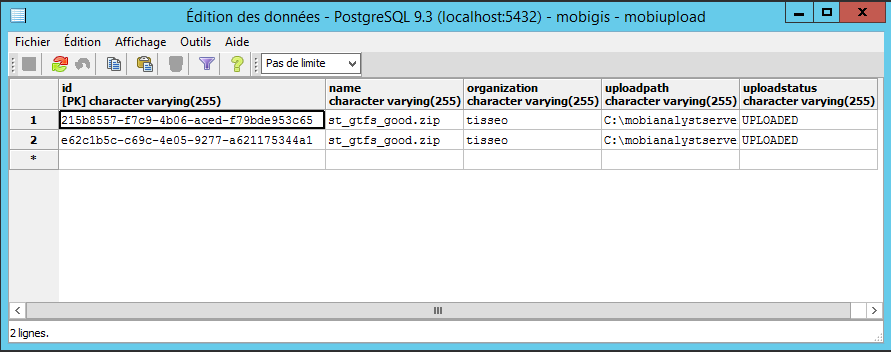
\includegraphics[width=14cm]{images/tablePostgres_mobiupload_small.png}
\caption{\label{TablePostgres}Table des uploads sur le SGBD PostgreSQL}
\end{figure} 

A chaque requête POST du client, je créé une instance d'objet Upload, les informations sont saisies dans la table de suivi, et je stocke les données envoyées sur le serveur. Pour chaque client ou utilisateur, pour chaque type de données, il y a un répertoire personnalisé, chaque upload est \og taggé \fg d'un identifiant unique \og UUID \fg.
Le code métier qui a été implémenté est pour le moment le test sur le type de données envoyées, la validation des données et la production d'un rapport d'un validation (JSON), enfin l'extraction (récursive) des données contenues dans l'archive (cf. Annexe \ref{Annexe D}).\\

A partir de ce service spécifique, dédié aux données GTFS, j'ai généralisé cette resource (FileResource.java) afin de permettre d'upload n'importe quel fichier sur le serveur, en réutilisant les mêmes méthodes, notamment celle de UploadDAO.java et la méthode \og métier \fg manageUpload().\\

Dans un deuxième temps, j'ai entamé la fonctionnalité de chargement en base et permettre la persistance des données GTFS au sein de la base de données Postgres. A partir des classes du modèle (package gtfs) (Fig \ref{packageGTFS}), et du schéma relationnel  (Fig \ref{RelationalGTFS}), j'ai produit à l'aide des annotations JPA le code nécessaire à la génération du schéma gtfs dans la base et le chargement des données (txt).\\
\begin{figure}[!h]
\centering
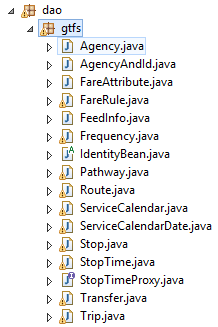
\includegraphics[width=6cm]{images/model_GTFS.PNG}
\caption{\label{packageGTFS}Classes des objets GTFS (couche modèle)}
\end{figure}

\begin{figure}[!h]
\centering
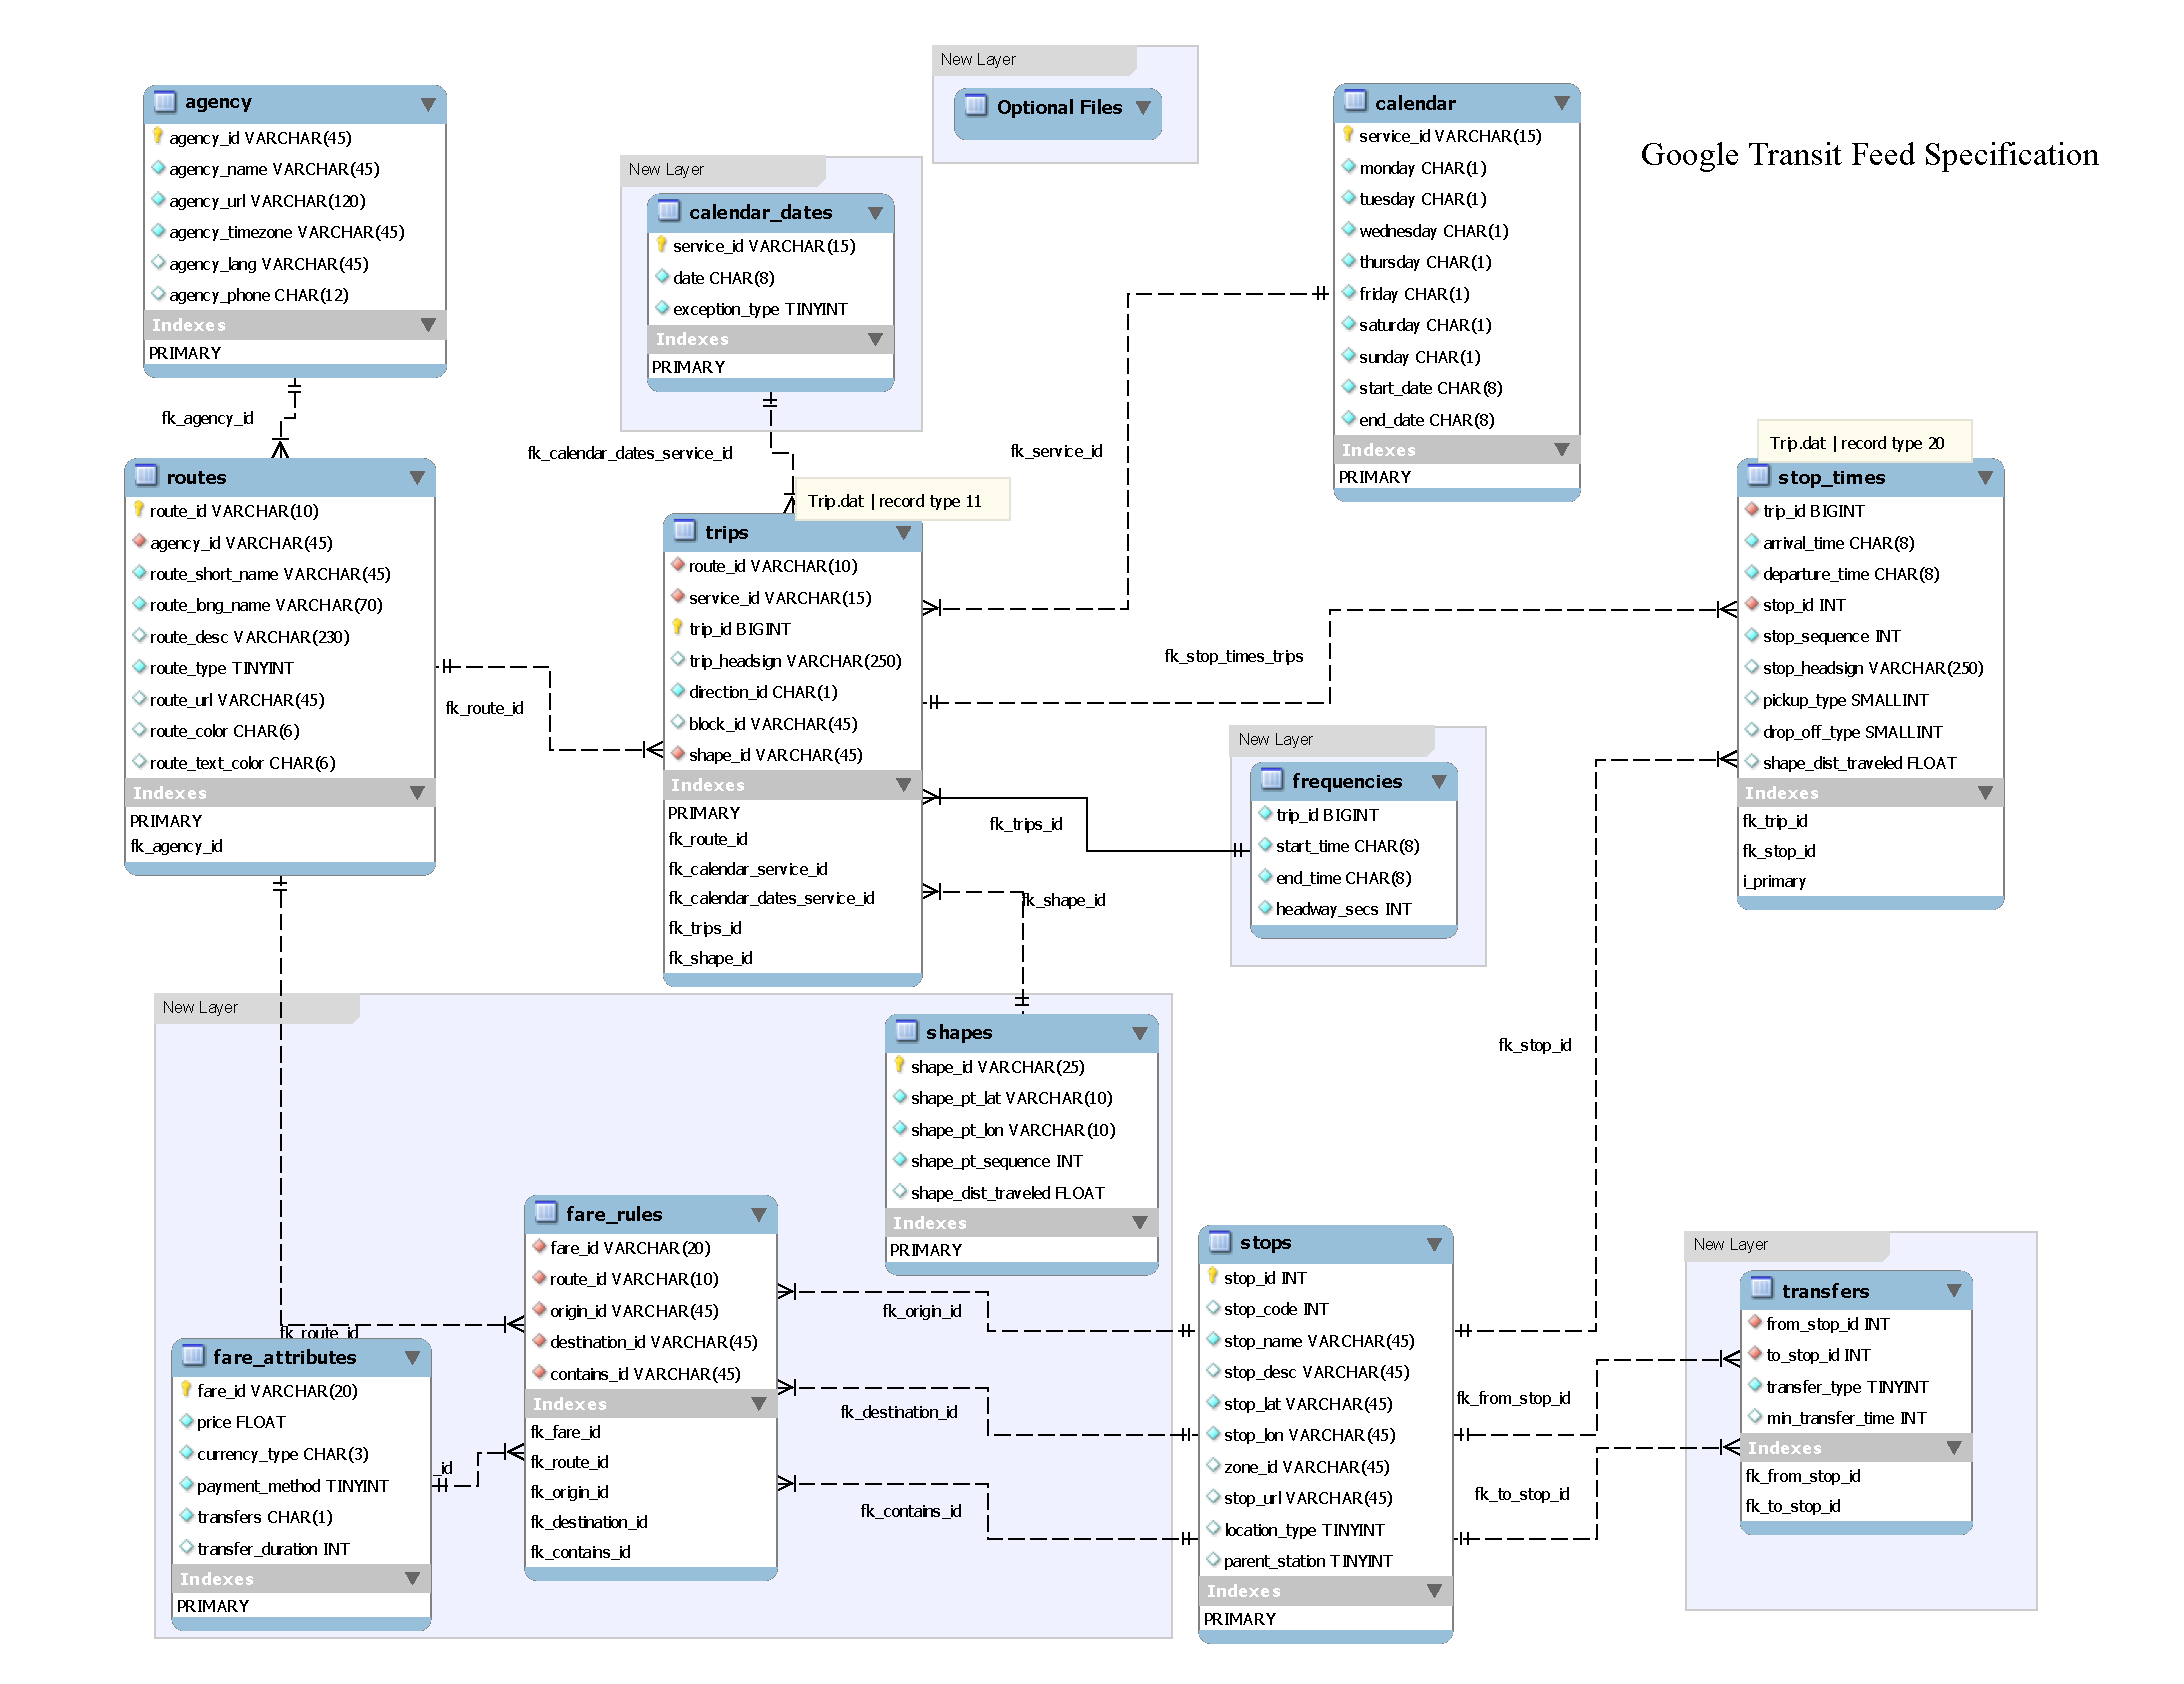
\includegraphics[width=14cm]{images/GTFS_Schema.png}
\caption{\label{RelationalGTFS}Modèle relationnel des données GTFS (couche modèle)}
\end{figure}


\paragraph{Application multi-couches :}
~\\
~\\
\textbf{Domaine métier}\\

Les classes du domaine métier sont des POJOs (Plain Old Java Object) et sont persistés par les objets d'accès aux données (DAO : Data Access Object). L'acronyme POJO est principalement utilisé pour faire référence à la simplicité d'utilisation d'un objet Java en comparaison avec la lourdeur d'utilisation d'un composant EJB. Ainsi, un POJO n'implémente pas d'interface spécifique à un framework comme c'est le cas par exemple pour un composant EJB.\\

Voici l'exemple d'un objet (Upload.java) persisté par Hibernate : (cf. Annexe \ref{Annexe B})\\

Les annotations ne sont pas obligatoires et dépendent du framework de persistence utilisé.
Dropwizard n'apporte pas de restriction sur le choix de la librairie utilisée et apporte par défaut JDBI (module dropwizard-jdbi) et Hibernate (module dropwizard-hibernate).\\

\textbf{DAO}\\

La DAO UploadDAO étend la classe abstraite \textit{AbstractDAO} de Dropwizard pour avoir accès à Hibernate au travers de ces méthodes.\\

Voici l'exemple d'une classe DAO (UploadDAO.java) : (cf. Annexe \ref{Annexe C})\\

\textbf{Service REST}\\

La classe du service REST est autonome: il n'y a pas d'adhérence à Dropwizard. Elle utilise directement les annotations de Jersey: @Path, @Produces, @GET et quelques annotations de Dropwizard : @UnitOfWork, @LongParam... \\

La DAO UploadDAO est injectée via le constructeur. Cela a été effectuée dans la méthode run de la classe principale MobiSAASApplication de l'application Mobi-Admin via la ligne :
\item environment.jersey().register(new GtfsResource(dao));
\\


\paragraph{Programmation concurrente}\\ \label{Threads}
~\\

Un processus représente l'environnement d'exécution d'un programme. Il référence d'une part un espace mémoire permettant de stocker les données propres à l'application, et d'autre part un ensemble de threads permettant l'exécution du code qui manipulera ces données.\\

En Java, au démarrage de l'application, un thread initial est créé : le thread \og main \fg. Son rôle est de localiser le point d'entrée de l'application (la méthode public static void main(String... args)) puis d'exécuter son code.
Ce thread, comme tous les threads, exécute la séquence d'instructions qui lui est confiée de manière purement séquentielle. Si une instruction prend du temps à compléter (par exemple, en attente de connexion à un serveur), toute l'application est paralysée.
Pour éviter cela, il est souhaitable de confier l'exécution de ces portions bloquantes à des threads annexes, laissant ainsi le thread principal libre de continuer l'exécution de l'application.\\

\textbf{Le framework \og Executor \fg}\\
~\\
Disponible dans le package java.util.concurrent, il fournit un pool de threads robuste et hautement configurable, ainsi que les classes Callable et Future qui étendent les fonctionnalités des Runnables (approche plus classique?). Sa mise en œuvre doit systématiquement être préférée à la création manuelle de threads. Ce framework répond aux problématiques suivantes :
1> d'une part, chaque thread supplémentaire augmente la mémoire consommée, la complexité globale de l'application, et le risque de contention ;
2> d'autre part, pour de petites tâches, le coût de création d'un nouveau thread peut se révéler supérieur au coût d'exécution du traitement associé.\\

La méthode newFixedThreadPool() du service Executor permet de précharger en cache une réserve (pool) de threads et limite à un nombre fixe le nombre de requête simultanée (pour notre service le maximum est mis à 10). Ainsi, jusqu'à 10 requêtes, le service répondra et les traitements seront exécutés en parallèle, au-delà, la requête sera mise dans la file d'attente.\\

Afin de renvoyer un résultat et de savoir si le traitement lève une exception, le framework \og Executor \fg propose l'interface Callable<V>, qui est une sorte de Runnable amélioré. Le type paramétré <V> définit le type du résultat produit par la méthode call(). Ainsi, un Callable<String> produira un String.(Fig. \ref{UML1})\\

Une fois soumis à un pool de threads, un Callable est généralement exécuté de manière asynchrone ; le résultat produit ne sera sans doute pas disponible avant un certain temps.
Du point de vue de l'appelant (celui qui soumet le traitement au pool), cela n'aurait aucun sens d'attendre ce résultat de manière synchrone : il perdrait tout le bénéfice du système ! Mais il lui faut tout de même un moyen de récupérer le résultat lorsqu'il aura été calculé.

Le framework \og Executor \fg fournit donc la classe Future<V>, qui représente un résultat de type V dont la valeur est pour l'instant inconnue (puisque le traitement n'a pas encore été exécuté), mais qui sera disponible dans le futur. 
La méthode get() permet de récupérer le résultat immédiatement s'il est disponible (c'est-à-dire si le traitement a bien été exécuté par le pool de threads). Mais attention : si son calcul n'est pas terminé, la méthode est bloquante ! C'est donc une bonne pratique de vérifier la réelle disponibilité du résultat avec isDone() avant de le récupérer. \\



\paragraph{Tests}

Afin de tester les web services REST développés, j'ai utilisé fréquemment l'outil \textbf{SoapUI} (Fig. \ref{SoapUIGet}). Il permet de mettre en place une suite de tests qui peuvent être lancés d'une traite du côté client, permet de tester les services web en mode bouchon mais aussi d'effectuer des tests de charge. Il permet entre autre de fournir une hiérarchie des services web, de lister les différentes méthodes disponible, les paramètres attendus, de réaliser des requêtes et de récupérer les réponses … C'est l'un des meilleurs outils de test unitaires concernant les services web.\\

\begin{center}
\begin{figure}[h] \centering
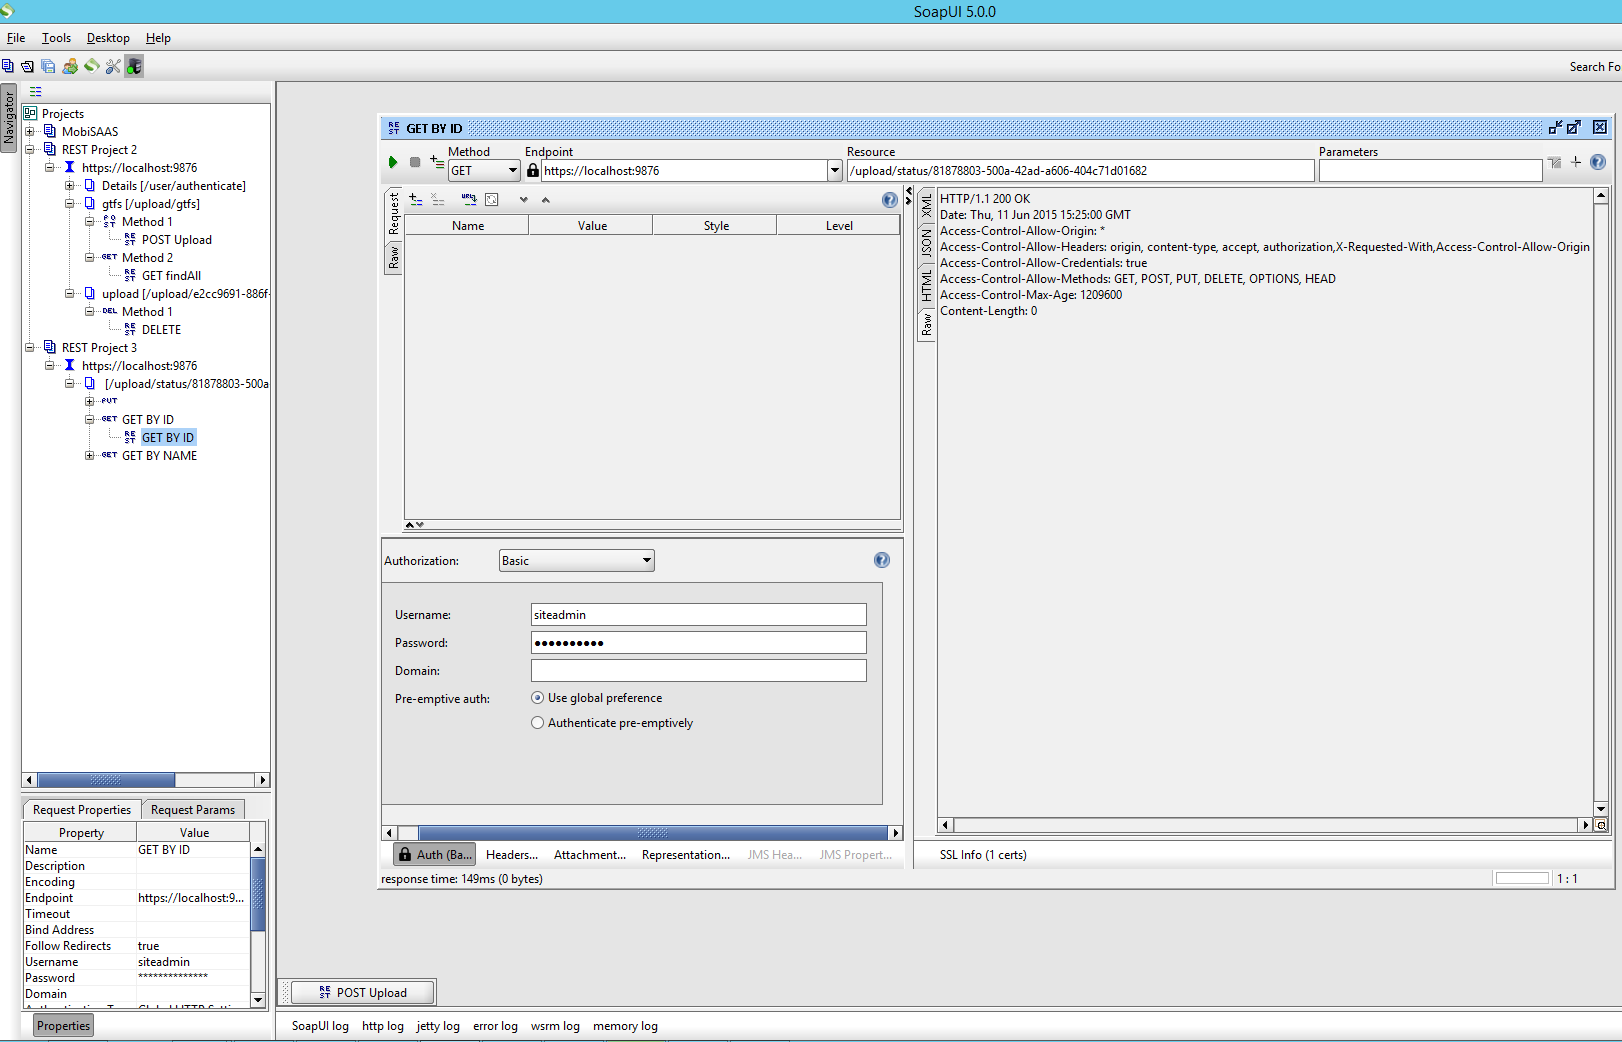
\includegraphics[width=16cm]{images/soapUI_getById_sansResponse_small.png}\\
\caption{\label{SoapUIGet} Interface et exemple de requête \og GET \fg SoapUI}
\end{figure}
\end{center}


\subsection{Perspectives}

L'idéal d'un programme développé dans un langage orienté objet est la généricité et la réutilisation d'un maximum de composants. Dans ce travail, l'objectif est clairement de produire un maximum de composants abstraits (classes et interfaces) et de méthodes réutilisables. 
Les perspectives du projet \og MobiSAAS \fg sont nombreuses : gérer une architecture distribuée, augmenter les fonctionnalités SAAS notamment les fonctionnalités de \og MobiAnalyst \fg, étendre le projet \og DataWizard \fg lui aussi en mode SAAS.\\

J'ai donc \og maquetté l'application \fg et débuté le développement de ces composants abstraits (ex: Les ressources au sens DropWizard (Fig. \ref{UML1}). Grâce à cela on pourra donc \og uploader \fg plusieurs types de données et réutiliser la méthode manageUpload(). Egalement, sur ce même principe j'ai développé une classe abstraite afin de faire proposer la gestion de l'asynchronisme utilisée dans tous les services que j'ai implémentés, limitant ainsi la duplication de codes dans l'application.\\

\begin{figure}[!h]
\centering
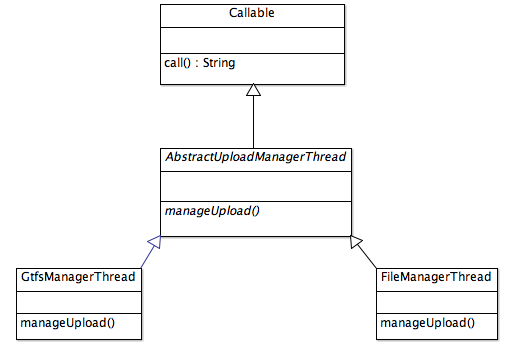
\includegraphics[width=14cm]{images/DiagrammeThread.png}
\caption{\label{UML1}Exemple d'abstraction et d'héritage de méthode}
\end{figure} 

J'ai commencé un autre traitement de données spécifique au format GTFS. Une méthode de chargement des données dans la base de données Postgresql (méthode loadData()). J'utilise pour cela une librairie appelée OneBusAway\footnote{\url{http://onebusaway.org/developer-information/}} (OBA) spécialisée dans le transport en commun. Ce traitement réalise une désérialisation (lecture de fichiers csv) et une persistance des données via le framework Hibernate dans Postgresql. Ce qu'il reste à faire est de passer la méthode en service REST.\\





\pagebreak

\section{DataWizard}\label{DataWizard}

\subsection{Cahier des charges}

\subsubsection{Présentation des besoins}

Le projet \og DataWizard \fg, ensemble de scripts Python et SQL est une application dont le but est d'ingérer des données de transports, et de voirie dans une base de données spatiales (\textbf{PostGIS}\ref{Postgis}) afin de produire en sortie un réseau de transport (Network Dataset ou NDS).\\
Sur ce projet, les besoins correspondent à des corrections de bugs ainsi que des développements d'évolutions de fonctionnalités décrites sur le projet Redmine. Ainsi, j'ai réalisé de la production (nombreux réseaux), et j'ai fait évoluer l'outil notamment afin de lui permettre de produire des métadonnées.\\


\subsection{Eléments de spécifications fonctionnelles}

Le DataWizard permet de se lancer par étapes. Il y a 10 étapes successives, dont une étape préliminaire appelée étape 0, et une indépendante : l'étape 10.\\
\begin{itemize}
\item STEP 0 : Nettoyage et préparation de la base de données
\item STEP 1 : Import des données transport en commun et conversion vers le schéma mobianalyst
\item STEP 2 : Import des données de voirie
\item STEP 3 : Import des données métro et conversion vers le schéma mobianalyst
\item STEP 4 : Génération des données vitesses moyennes et horaires et connexion des réseaux de transport en commun et voirie
\item STEP 5 : Calcul des horaires et des vitesses moyennes
\item STEP 6 : Export des données vers des fichiers Shapefile (.shp)
\item STEP 7 : Import des données dans la Géodatabase de sortie et changement du système de projection si nécessaire
\item STEP 8 : Extraction des différents modes, génération du fichier xml servant à construire le réseau et de MobiNetwork.xml
\item STEP 9 : Construction et compilation du réseau
\item STEP 10 : Production de métadonnées pour le réseau
\end{itemize}

Afin de fournir, un réseau conforme aux attentes du logiciel MobiAnalyst \og version 3.0 \fg et des experts en analyse de réseaux de transports, l'équipe me fournit une spécification de métadonnées à extraire des données en entrée du DataWizard (Fig. \ref{DW_Metadata}).\\

\begin{figure}[!h]
\centering
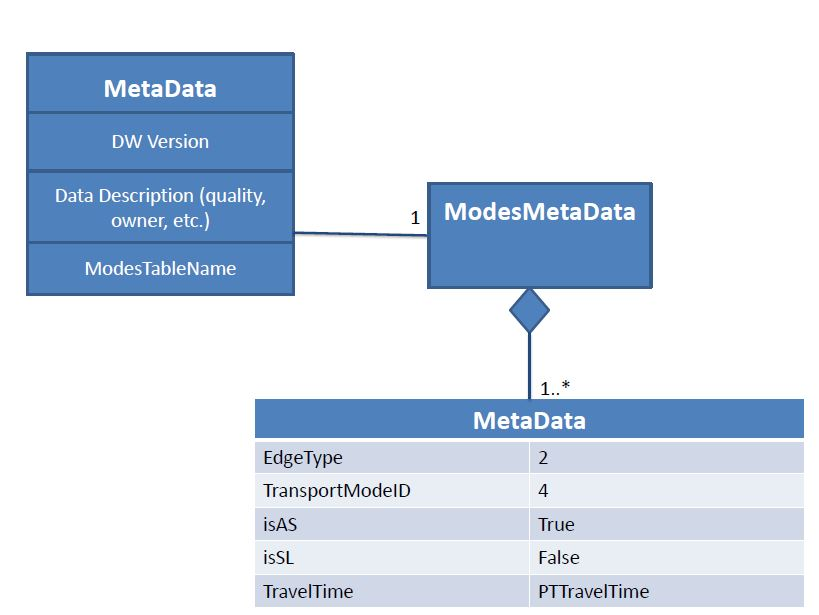
\includegraphics[width=12cm]{images/DW_specMetadata.JPG}
\caption{\label{DW_Metadata}Métadonnées de réseau de transports v3.0}
\end{figure} 

\subsection{Eléments de spécifications techniques}

J'intègre tout d'abord le projet en tant qu'utilisateur, j'exploite des données et produits des réseaux de transport en commun (TC) (Bordeaux, Champagne-Ardennes, Montreal, Melbourne,etc.). Ensuite, petit à petit je suis le plan de charge issu du projet Redmine et corrige des bugs et des anomalies.\\

Mon premier travail a été de développer l'étape 10 (STEP 10 : Export Metadata Tables) de l'exécution du DataWizard. Pour cela j'ai du extraire le nombre de modes de transport en commun (variable selon chaque projet), leurs codes (variable selon chaque projet) et enfin extraire des listes de constantes pour documenter le réseau produit par le DataWizard.\\

Un autre travail réalisé est le développement qui permet la gestion du système de projection des données géographiques pour les calculs du DataWizard. Cette modification impacte quasiment la totalité des requêtes SQL dites spatiales de l'application, et permet des résultats (calculs de distances) plus réalistes (par exemple pour Melbourne, Australie située dans l'hémisphère Sud).\\


\subsection{Réalisations}

Les principales difficultés concernent les données. Ces données GTFS ou voirie (données Here\footnote{\url{https://company.here.com/here/}} (anciennement Navteq) ou OpenStreetMap\footnote{\url{http://openstreetmap.fr/}}) sont complexes. La base de données \og DataWizard \fg possède ainsi de nombreux schémas, et les requêtes SQL sont parfois très complexes mêlant fonctions, et requêtes géographiques.\\

Les résultats obtenus sont la production de nombreux réseaux avec leurs métadonnées pour nos analystes, et pour les projets de R\&D nécessitant des réseaux récents (Moveazy, Mobilyse, etc...). J'ai ainsi amélioré la stabilité de l'application.\\

Exemple de code pour produire une table de métadonnées (Fig. \ref{CodeMetadata}) :
\\
\begin{figure}[h]
	\centering
		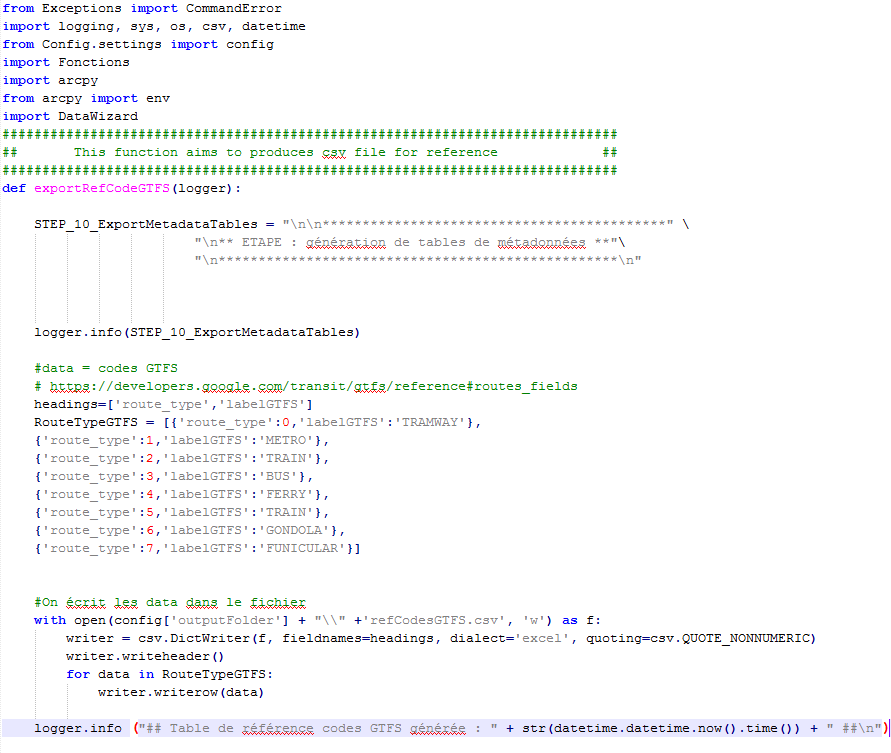
\includegraphics[width=0.8\textwidth]{images/DW_Fonction_Python.PNG}
	\caption{Fonction Python pour exporter des métadonnées}
	\label{CodeMetadata}
\end{figure}\\

Dans ce projet, j'ai également développé des fonctions utilitaires : BOMConverter.py, searchAndReplaceFiles.py, etc... Ces méthodes permettent notamment de formater les données avant leur import dans la base de données. Cela peut certainement éviter les mauvaises surprises d'encodage ou de caractères spéciaux fréquemment rencontrés lors de l'exploitation de données GTFS.\\



\subsection{Perspectives}

La liste des évolutions sur le projet Redmine est longue, il y a en effet énormément de perspectives pour le projet... Tout d'abord permettre l'import de plusieurs formats de données, comme l'import de données \og Shapefile \fg qui n'est pas encore terminé, mais aussi de données de transports en commun \og Trident \fg, de données de traffic, etc. 
Augmenter encore la capacité de l'outil à rendre ses étapes indépendantes, nettoyer les fonctions obsolètes, revoir l'algorithme de certaines méthodes,...
D'une manière générale les besoins pour l'application sont d'optimiser les étapes longues, et de développer des routines de simplification de données (SQL) afin par exemple de ne retenir que les données nécessaires au traitement au lieu de charger toutes les données en amont, réalisé des tests de qualité sur les données d'entrée... \\

A long terme, l'idée est de proposer toutes les fonctionnalités du DataWizard via une application en mode SAAS.\\


\section{Crislab}\label{Divers}

\subsection{Présentation} 

Ce projet est dédié à la Cartographie des RISques de LABoratoire. Il consiste en une application web, proposant une interface cartographique des bâtiments afin de permettre la gestion des marqueurs et relevés de zones à risques. La vocation de l'application est un site intranet. Durant mon stage, j'ai eu de nombreux échanges avec le client afin de résoudre des bugs de l'application. J'ai donc participé au débugage et à la production de nouveaux livrables (.war).\\

Le projet est très complet, et présente une architecture assez typique d'une application web (cf. Annexe \ref{Annexe C}). Ainsi, l'interface Homme-Machine (IHM) est codée en Javascript, il y a de nombreux formulaires d'affichage ou de saisie dans des fichiers JSP  (Java Server Pages), la partie cartographique est encore une fois produite par un serveur ArcGIS dédié. Le serveur d'applications est un serveur Tomcat 6, adossé sur un SGBD Oracle 10g. Toute la persistance est gérée via le framework Hibernate.\\

\begin{figure}[h]
	\centering
		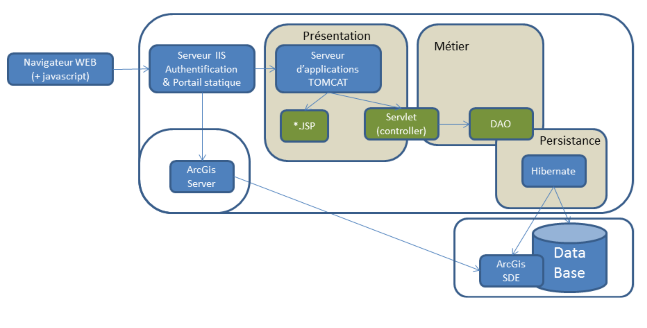
\includegraphics[width=0.8\textwidth]{images/Architecture_Crislab.PNG}
	\caption{Architecture globale de l'application Crislab}
	\label{fig:architecture}
\end{figure}\\


\subsection{Réalisations}

J'ai donc \og administré \fg le projet sous Eclipse avec Maven, j'ai lancé l'application sur un serveur Tomcat, créé différents profils de configuration (développement, tests, production) avec des propriétés de connexion différentes à chaque profil). J'ai testé l'application avec le navigateur \og client \fg Internet Explorer 11. Ce projet m'a permis de mettre en application mes connaissances client-serveur, sur toute la partie présentation d'une application web depuis l'affichage des JSP jusqu'aux actions déclenchées (couche service) interceptées par les contrôleurs.\\

Le debug a surtout consisté à reproduire les bugs de l'application en production. Du coup, j'ai du importer le schéma de la base de données (Oracle) des clients, tester les requêtes de mon service sur leurs données. J'ai essentiellement passé mon temps à refaire les requêtes, et notamment traduire le HQL (langage de requête Hibernate) en SQL (langage de requête \og standard \fg). Par exemple, le premier bug était du à une mauvaise initialisation d'une variable. Un deuxième bug venait  d'une mauvaise manipulation de l'opérateur qui avait provoqué la création d'un doublon dans la base (chose impossible à réaliser via l'interface cliente (IHM)).\\
